\documentclass[notes,11pt,aspectratio=169]{beamer}

\usepackage{amsmath}
\usepackage{amssymb}
\usepackage{amsfonts}
\usepackage{booktabs}
\usepackage{threeparttable}
\usepackage{graphicx}
\usepackage{adjustbox}
\usepackage{xspace}
\usepackage{appendixnumberbeamer}

\usepackage[
  backend=biber,
  style=authoryear,
  maxcitenames=2,
  mincitenames=1,
  maxbibnames=10,
  minbibnames=1,
  uniquelist=false,
  uniquename=false
]{biblatex}

\let\oldparencite\parencite
\renewcommand{\parencite}[2][]{%
  \footnotesize {\tiny \oldparencite[#1]{#2}} \normalsize %
}

\renewcommand*{\bibfont}{\footnotesize}

\addbibresource{causal_effect_schools.bib}

\usetheme[progressbar=frametitle]{metropolis}

\newcommand{\blue}[1]{\textcolor{blue}{#1}}
\newcommand{\red}[1]{\textcolor{red}{#1}}
\newcommand{\green}[1]{\textcolor{teal}{#1}}

\newenvironment{wideitemize}{%
  \begin{minipage}{0.90\textwidth}
  \begin{itemize}
  \addtolength{\itemsep}{1em}
}{%
  \end{itemize}
  \end{minipage}
}

\newenvironment{cwideitemize}{%
  \begin{center}
  \begin{minipage}{0.90\textwidth}
  \begin{itemize}
  \addtolength{\itemsep}{1em}
}{%
  \end{itemize}
  \end{minipage}
  \end{center}
}

\title{\texorpdfstring{\centering{How Much Do High Schools Matter?\\[0.35em]
Causal Effects on Achievement and Major Choice} \\ }{How Much Do High Schools Matter? Causal Effects on Achievement and Major Choice}}
\author[BEAM]{%
  \texorpdfstring{%
    \begin{columns}
      \column{.3\linewidth}
      \centering
      \column{.3\linewidth}
      \centering
      Bruno E. Aravena-Maguida\\ UChicago
      \column{.3\linewidth}
      \centering
    \end{columns}
  }
  {BEAM}
}
\date{\vspace{20pt}\hfill August 2026}

\begin{document}

\maketitle

\section{Motivation}

\begin{frame}{Question}
\begin{cwideitemize}
  \item How much do high schools matter for students' later achievement and higher-education choices?

  \item The school-effects literature has strong evidence on achievement, but much less on whether schools affect field of study and the quality of the higher-education match. \parencite{angrist_stand_2016,dobbie_medium-term_2015,angrist_leveraging_2017,angrist_credible_2024}

  \item The practical challenge is that ``school attended'' is a high-dimensional treatment: one treatment for each high school.
\end{cwideitemize}
\end{frame}

\begin{frame}{What Changed Since the March Version}
\begin{wideitemize}
  \item March version: replicate the Chilean assignment system and use lottery offers/risk to estimate school-specific reduced-form effects.

  \item Spring pivot: replace the many-school treatment with a scalar school-value treatment.

  \item Current version: make the scalar design computationally tractable with expected-risk controls and reduce noisy school-value estimates with Empirical-Bayes shrinkage.

  \item The outcome set now extends beyond scores and STEM enrollment to higher-ed enrollment, accreditation, and program-income measures.
\end{wideitemize}
\end{frame}

\begin{frame}{Original Problem: Many Treatments}
\begin{wideitemize}
  \item A fully flexible treatment would include one indicator for each high school:
  \[
    D_i^{\mathrm{full}}
    =
    \left(
    \mathbf{1}\{S_i=1\},
    \mathbf{1}\{S_i=2\},
    \ldots,
    \mathbf{1}\{S_i=J\}
    \right).
  \]

  \item The lottery shifts students across schools, but generally does not identify a separate causal effect for every school.

  \item Students also have different next-best alternatives, so target-school effects are not automatically comparable.
\end{wideitemize}
\end{frame}

\begin{frame}{Different Fallbacks}
\begin{wideitemize}
  \item If all students had the same guaranteed fallback \(G\), lottery-induced comparisons could be interpreted as
  \[
    \beta_{AG}, \qquad \beta_{BG}, \qquad \beta_{CG}.
  \]

  \item In practice, students have different fallback schools:
  \[
    G_i \in \{G^1, G^2, \ldots, G^K\}.
  \]

  \item The relevant objects become target-school-by-fallback effects:
  \[
    \beta_{AG^1}, \beta_{AG^2}, \ldots, \beta_{CG^K}.
  \]

  \item This motivates projecting school attendance into a scalar school-value index.
\end{wideitemize}
\end{frame}

\begin{frame}{A Related Move: Next-Best Effects}
\begin{wideitemize}
  \item \textcite{kirkeboen_field_2016} study field-of-study effects using centralized assignment in Norway.

  \item Their solution is to collapse programs into broad fields and estimate next-best effects across fields.

  \item The cost is that their main specification abstracts away from institution-level variation.

  \item My current approach keeps school-level variation, but projects it onto a pre-specified continuous margin.
\end{wideitemize}
\end{frame}

\begin{frame}{Next-Best Effects in Practice}
\begin{figure}
  \centering
  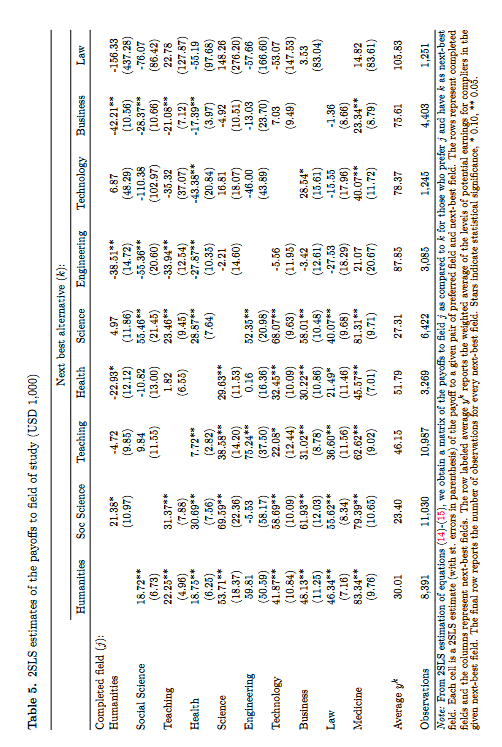
\includegraphics[width=1.2\linewidth,height=1.2\textheight,keepaspectratio,angle=270]{magne_table.png}
\end{figure}
\vspace{-0.8em}
\begin{center}
  \tiny Source: \oldparencite{kirkeboen_field_2016}.
\end{center}
\end{frame}

\begin{frame}{Main Object}
\begin{wideitemize}
  \item For each school \(s\), construct a school-value index \(V_s^m\) for metric \(m\).

  \item A student's endogenous treatment is the value of the school they attend:
  \[
    A_i^m = V_{S_i}^m.
  \]

  \item The instrument is the value of the school offered by the lottery:
  \[
    O_i^m = V_{R_i}^m.
  \]

  \item The IV asks whether lottery-induced movement toward higher-value schools causally improves outcomes.
\end{wideitemize}
\end{frame}

\section{Data and School Values}

\begin{frame}{Data}
\begin{wideitemize}
  \item Universe: students observed in regular grade 8 in Chile between 2017 and 2020.

  \item Approx. 944,000 unique students.

  \item Linked records:
  \begin{itemize}
    \item grade-4 SIMCE math and language scores;
    \item grade-8 cohort, gender, age, and home comuna;
    \item centralized assignment probabilities and lottery offers;
    \item high-school enrollment histories after grade 8;
    \item PSU/PAES math and language scores;
    \item higher-education enrollment, fields, accreditation, and program-income measures.
  \end{itemize}
\end{wideitemize}
\end{frame}

\begin{frame}{Assigning a High School}
\begin{wideitemize}
  \item For each student, I track school enrollment during the four years after grade 8.

  \item Main school assignment:
  \[
    S_i = \text{school code attended for the most post-grade-8 years}.
  \]

  \item Ties are broken toward the most recent school.

  \item This maps each student in the broad grade-8 universe to one high-school code when available.
\end{wideitemize}
\end{frame}

\begin{frame}{Raw and Adjusted School Values}
\small
\textbf{Raw school mean}
\[
V_s^{\mathrm{raw},m}
=
\frac{1}{N_s}
\sum_{i:S_i=s}Y_i^m.
\]

\vspace{0.5em}
\textbf{Adjusted observational value-added}
\[
Y_i^m
=
\mu
+
V_{S_i}^m
+
\sum_{p=1}^{3}\lambda_{Mp}M_i^p
+
\sum_{p=1}^{3}\lambda_{Lp}L_i^p
+
\gamma_{\mathrm{cohort}(i)}
+
\delta_{\mathrm{gender}(i)}
+
\rho_{\mathrm{age}(i)}
+
\kappa_{\mathrm{comuna}(i)}
+
\varepsilon_i .
\]

\vspace{0.2em}
\begin{itemize}
  \item \footnotesize \(V_s^m\) is a school fixed effect, interpreted as an observational and potentially selection-contaminated school-value metric. \parencite{chetty_measuring_2014,angrist_leveraging_2017}
\end{itemize}
\end{frame}

\begin{frame}{Adjustment Matters}
\begin{figure}
  \centering
  
\includegraphics[width=0.82\linewidth]{C:/Users/xd-br/Desktop/PhD/Research/causal_schools/output/figures/school_rbd_observational_values/math_values_by_region_raw_adjusted.png}
\end{figure}
\end{frame}

\section{Current IV Design}

\begin{frame}{Lottery Sample}
\begin{wideitemize}
  \item I use students who enter the grade-9 centralized assignment mechanism \textit{(SAE)} on time.

  \item I restrict to students with non-trivial assignment risk:
  \[
    \max_{s\in\mathcal{S}} p_{is}<1,
  \]
  where \(p_{is}\) is the simulated probability that student \(i\) is assigned to school \(s\).

  \item Current diagnostics: about 419,000 student-process rows, 163,600 timely at-risk rows, and 106,374 exam-taker timely at-risk rows.

  \item The offer provides exogenous variation in attended-school value, conditional on lottery risk.
\end{wideitemize}
\end{frame}

\begin{frame}{Previous Risk Controls}
\begin{wideitemize}
  \item The spring design used a supported school set and included two controls for each supported school:
  \begin{itemize}
    \item the probability of assignment to the school;
    \item an indicator for zero assignment probability.
  \end{itemize}

  \item With the 100-student support threshold, this meant roughly 2,000 risk controls.

  \item This was feasible for main estimates but costly for heterogeneity and extensions.
\end{wideitemize}
\end{frame}

\begin{frame}{Current Risk Control: Expected School Value}
\small
\[
E_i^m
=
\sum_s p_{is} V_s^m.
\]

\vspace{0.4em}
\begin{wideitemize}
  \item \(p_{is}\): simulated probability that student \(i\) is assigned to school \(s\).

  \item \(V_s^m\): school value for metric \(m\).

  \item Instead of controlling for the full probability vector, I control for the scalar expected value of the lottery risk set.

  \item This keeps the design close to the assignment-risk logic while making the current regressions much easier to run and extend.
\end{wideitemize}
\end{frame}

\begin{frame}{2SLS System}
\small
\[
A_i^m
=
\pi_0
+
\pi_1 O_i^m
+
\eta E_i^m
+
X_i'\lambda_D
+
u_i .
\]

\[
Y_i^m
=
\alpha
+
\theta \widehat{A}_i^m
+
\phi E_i^m
+
X_i'\lambda_Y
+
\varepsilon_i .
\]

\vspace{0.5em}
\begin{wideitemize}
  \item \(A_i^m\): value of the school attended after grade 8.
  \item \(O_i^m\): value of the first-round offered school.
  \item \(E_i^m\): expected school value under assignment probabilities.
  \item \(X_i\): cohort, gender, grade-8 age, grade-4 math, and grade-4 language controls.
\end{wideitemize}
\end{frame}

\section{Main Results}

\begin{frame}{How to Read \(\theta\)}
\begin{wideitemize}
  \item The coefficient \(\theta\) is a pass-through parameter from observational school value to lottery-induced causal gains.

  \item If a complier is induced to attend a school with one unit higher \(V_s^m\), their outcome is expected to move by \(\theta\) units.

  \item If \(\theta=1\), the observational school-value index maps one-for-one into the causal effect along the lottery margin. \parencite{angrist_leveraging_2017}
\end{wideitemize}
\end{frame}

\begin{frame}{Expected-VA Main Results}
\centering
\scriptsize
\begin{tabular}{lcccccc}
\toprule
 & \multicolumn{2}{c}{Math VA} & \multicolumn{2}{c}{Language VA} & \multicolumn{2}{c}{STEM VA} \\
\cmidrule(lr){2-3} \cmidrule(lr){4-5} \cmidrule(lr){6-7}
Specification & \(\theta\) & SE & \(\theta\) & SE & \(\theta\) & SE \\
\midrule
Unadjusted & 0.246 & 0.029 & 0.190 & 0.029 & 0.390 & 0.050 \\
Adjusted & 0.841 & 0.071 & 0.835 & 0.082 & 0.689 & 0.067 \\
\bottomrule
\end{tabular}

\vspace{0.8em}
\footnotesize
Expected-risk-control specification. Adjusted school values are much closer to one-for-one pass-through.
\end{frame}

\begin{frame}{Interpretation}
\begin{wideitemize}
  \item Observational school value predicts lottery-induced causal gains in achievement and STEM enrollment.

  \item Adjusted metrics perform substantially better than raw school means, consistent with selection bias in unadjusted values.

  \item The STEM result suggests that high schools affect higher-education major choice, not only test scores.

  \item The expected-risk-control design makes it easier to run heterogeneity and new-outcome exercises.
\end{wideitemize}
\end{frame}

\begin{frame}{Heterogeneity by Grade-4 Math Quintile}
\centering
\scriptsize
\begin{tabular}{lcccccc}
\toprule
 & \multicolumn{2}{c}{Math VA} & \multicolumn{2}{c}{Language VA} & \multicolumn{2}{c}{STEM VA} \\
\cmidrule(lr){2-3} \cmidrule(lr){4-5} \cmidrule(lr){6-7}
Grade-4 math quintile & \(\theta\) & SE & \(\theta\) & SE & \(\theta\) & SE \\
\midrule
Q1 & 0.145 & 0.145 & 0.596 & 0.180 & 0.735 & 0.132 \\
Q2 & 0.785 & 0.133 & 0.601 & 0.178 & 0.487 & 0.144 \\
Q3 & 0.940 & 0.151 & 0.929 & 0.188 & 0.955 & 0.153 \\
Q4 & 0.771 & 0.158 & 1.122 & 0.182 & 0.567 & 0.166 \\
Q5 & 1.317 & 0.166 & 0.891 & 0.184 & 0.707 & 0.163 \\
\bottomrule
\end{tabular}

\vspace{0.8em}
\footnotesize
Adjusted expected-VA estimates, full grade-4 SIMCE split.
\end{frame}

\begin{frame}{Higher-Education Quality Outcomes}
\centering
\scriptsize
\begin{tabular}{lcccc}
\toprule
 & \multicolumn{2}{c}{Program-certified years} & \multicolumn{2}{c}{Institution-certified years} \\
\cmidrule(lr){2-3} \cmidrule(lr){4-5}
Specification & \(\theta\) & SE & \(\theta\) & SE \\
\midrule
Unadjusted & 0.299 & 0.115 & 0.688 & 0.112 \\
Adjusted & 0.872 & 0.156 & 1.153 & 0.123 \\
\bottomrule
\end{tabular}

\vspace{0.8em}
\footnotesize
The scalar school-value framework also predicts lottery-induced movement into more accredited higher-education options.
\end{frame}

\section{Empirical-Bayes School Values}

\begin{frame}{Why Shrink School Values?}
\begin{wideitemize}
  \item School value-added estimates are noisy, especially for smaller schools and rarer outcomes.

  \item The current EB path shrinks first-stage observational school values before using them as the scalar school-quality index.

  \item This is not a new causal estimand. It validates an EB-shrunken observational school-value index along the SAE lottery margin.

  \item EB and non-EB \(\theta\)'s should be interpreted together with the scale of the underlying school-value index.
\end{wideitemize}
\end{frame}

\begin{frame}{EB Shrinkage}
\small
\[
\tau_m^2
=
\max\left\{
\widehat{\mathrm{Var}}_w(\widehat{V}_s^m)
-
\widehat{\mathbb{E}}_w\left[\widehat{\mathrm{se}}_s^{\,2}\right],
0
\right\}.
\]

\[
\lambda_s^m
=
\frac{\tau_m^2}{\tau_m^2+\widehat{\mathrm{se}}_s^{\,2}}.
\]

\[
V_{s,EB}^m
=
\bar{V}^m
+
\lambda_s^m
\left(
\widehat{V}_s^m-\bar{V}^m
\right).
\]

\vspace{0.2em}
\begin{wideitemize}
  \item Weights use the number of students in the school-value regression.
  \item Output is recentered to preserve the student-weighted zero-mean convention.
\end{wideitemize}
\end{frame}

\begin{frame}{EB Expected-VA IV}
\small
\[
A_i^{m,EB}=V_{S_i,EB}^m,
\qquad
O_i^{m,EB}=V_{R_i,EB}^m,
\qquad
E_i^{m,EB}=\sum_s p_{is}V_{s,EB}^m.
\]

\vspace{0.5em}
\begin{wideitemize}
  \item The IV specification is the same expected-risk-control design.

  \item The only change is replacing the raw adjusted school-value index with the EB-shrunken index.

  \item The mean assignment-probability mass covered by EB values is about 0.865 across the main metrics.
\end{wideitemize}
\end{frame}

\begin{frame}{EB Main Results}
\centering
\scriptsize
\begin{tabular}{lcccc}
\toprule
 & Math & Language & STEM enrollment & Institutional quality \\
\midrule
\(\theta^{EB}\) & 0.881 & 0.908 & 0.824 & 1.508 \\
SE & (0.074) & (0.089) & (0.080) & (0.166) \\
Observations & 90,906 & 92,472 & 92,959 & 92,959 \\
\bottomrule
\end{tabular}

\vspace{0.8em}
\footnotesize
EB-shrunken values preserve the core finding and make the main pass-through estimates close to one for test scores and STEM.
\end{frame}

\begin{frame}{Additional EB Outcomes}
\centering
\scriptsize
\begin{tabular}{lccc}
\toprule
 & Exam taking & Higher-ed enrollment & Program income \\
\midrule
\(\theta^{EB}\) & 0.478 & 0.748 & 1.316 \\
SE & (0.053) & (0.117) & (0.154) \\
Observations & 135,898 & 135,898 & 92,959 \\
\bottomrule
\end{tabular}

\vspace{0.8em}
\footnotesize
Current evidence points to effects on participation in the higher-education pipeline and on the value of the eventual program match.
\end{frame}

\begin{frame}{Program-Income Components}
\centering
\scriptsize
\begin{tabular}{lccc}
\toprule
 & Program income: area FE & Program income: institution FE & Program income: full \\
\midrule
\(\theta^{EB}\) & 1.118 & 1.327 & 1.084 \\
SE & (0.144) & (0.167) & (0.133) \\
Observations & 92,959 & 92,959 & 92,959 \\
\bottomrule
\end{tabular}

\vspace{0.8em}
\footnotesize
The program-income exercise separates broad field composition from institution-level and full program-income measures.
\end{frame}

\begin{frame}{Decomposing Full Program-Income VA}
\begin{wideitemize}
  \item I decompose school-level full program-income VA into orthogonal components.

  \item Current preferred ordering under consideration:
  \[
    \text{exam taking}
    \rightarrow
    \text{math}
    \rightarrow
    \text{area income}
    \rightarrow
    \text{institution income}.
  \]

  \item This asks whether schools shift students toward higher-income programs through exam participation, achievement, field composition, institution choice, or residual channels.
\end{wideitemize}
\end{frame}

\begin{frame}{Decomposition: Exam-First Version}
\centering
\scriptsize
\begin{tabular}{lcccc}
\toprule
 & Exam-taking component & Math component & Institution component & Area component \\
\midrule
\(\theta^{EB}\) & -2.003 & 0.426 & -0.022 & 1.152 \\
SE & (0.566) & (0.435) & (0.762) & (0.130) \\
Observations & 92,958 & 92,958 & 92,958 & 92,958 \\
\bottomrule
\end{tabular}

\vspace{0.8em}
\footnotesize
Preliminary scalar-component results suggest the area/field component is the clearest positive channel in this ordering.
\end{frame}

\section{Where This Leaves the Project}

\begin{frame}{Current Takeaways}
\begin{wideitemize}
  \item The scalar school-value approach makes the assignment lottery usable without estimating one treatment effect for every high school.

  \item Expected-VA risk controls make the design substantially more scalable.

  \item Adjusted and EB-shrunken school values predict lottery-induced gains in scores, STEM enrollment, accreditation, and program-income measures.

  \item The results are consistent with high schools affecting higher-education trajectories beyond achievement alone.
\end{wideitemize}
\end{frame}

\begin{frame}{Remaining Interpretation Work}
\begin{wideitemize}
  \item Clarify exactly what pass-through parameter is identified when the school-value index is noisy or shrunken.

  \item Compare EB and non-EB results in units that account for the SD of each school-value index.

  \item Decide whether the expected-VA risk-control design is the main specification or a scalable complement to the high-dimensional risk controls.

  \item Refine the program-income decomposition and decide which component ordering is most defensible.
\end{wideitemize}
\end{frame}

\begin{frame}{Next Short-Term Steps}
\begin{wideitemize}
  \item Formalize the expected-risk-control estimand and its relation to the earlier probability-control specification.

  \item Add scale diagnostics for EB versus non-EB school-value indices.

  \item Finish pooled interaction tests for gender and baseline-achievement heterogeneity.

  \item Turn the program-income decomposition into a more explicit mechanism exercise.
\end{wideitemize}
\end{frame}

\begin{frame}[standout]
Thanks!
\end{frame}

\end{document}
